\documentclass[12 pt]{article}
\usepackage{inputenc, amsmath, mathtools, xfrac, amssymb, graphicx, subfloat, IEEEtrantools, ulem, chngcntr, bm, enumerate}

\usepackage[letterpaper,margin=2.5cm]{geometry} % set the page parameters suitably
\setlength{\parskip}{0pt}
\counterwithin*{equation}{section}

\author{Gesha Mahendra Cunyadha - 1906348214}
\date{TA 2021-2022 Semester 5}
\title{Tugas Mandiri-Fisika Statistik}

\makeatletter 
\renewcommand{\thefigure}{\@arabic\c@figure}
\makeatother

\newcommand{\dbar}{d\hspace*{-0.08em}\bar{}\hspace*{0.1em}}

\usepackage[belowskip=1pt,aboveskip=0pt]{caption}%====
\captionsetup[figure]{name=Gambar}%===================== Mengatur jarak section & subsection
\setlength{\intextsep}{10pt plus 2pt minus 2pt}%========

\begin{document}
    \begin{titlepage}
        \begin{figure}
            \begin{center}
                
\includegraphics[width=2.5cm]{pic/makara.png}
            \end{center}
        \end{figure}  
        \maketitle
        \thispagestyle{empty}
    \end{titlepage}

    \pagenumbering{arabic}

    \title{\centering\Large{{\textbf{Soal}}}}

\textbf{Tugas 1 (Bab 1)}
    \begin{enumerate}
        \item Pandang gerak random $p=q$ dan $m=n_1-n_2$ menyatakan perpindahan ke kanan. Setelah jumlah total langakh $N$. Hitung:
        \begin{enumerate}[(a)]
            \item Hitung rata-rata $\overline{m}$, dan $\overline{m^3}$
            \item itung nilai rata-rata $\overline{m^2}$ dan $\overline{m^4}$
        \end{enumerate}
        \item Probabilitas $W(n)$ dinyatakan dengan probabilitas $p$ terjadi nilai $n$ kali dalam kejadian $N$ dinyatakan dengan distribusi Binomial
        \begin{equation*}
            W(n)=\dfrac{N!}{n!(N-n)!}p^n(1-p)^{N-n}
        \end{equation*}
        Perimbangkan kondisi ketika $p\ll 1$ dan $n\ll N$
        \begin{enumerate}[(a)]
            \item Jika $\ln(1-p)\approx-p$. Tunjukkan $(1-p)^{N-n}$
            \item Tunjukkan bahwa $\dfrac{N!}{(N-n)!}\approx N^n$
            \item Tunjukkan bahwa $W(n)=\dfrac{\lambda^n}{(n!)e^{-\lambda}}$ dengan $\lambda=Np$ dikenal sebagai distribusi Poisson.
        \end{enumerate}
        \item Pandang distribusi Poisson
        \begin{enumerate}[(a)]
            \item Tunjukkan sifat normalisasi $\sum_{n=0}^N W_n=1$
            \item Hitung nilai $\overline{n}$
            \item Hitung nilai $\overline{(\Delta n)^2}\equiv\overline{(n-\overline{n})^2}$
        \end{enumerate}
    \end{enumerate}
\textbf{Tugas 2 (Bab 2)}
    \begin{enumerate}
        \item Sebuah partikel bermassa $m$ bergerak bebas dalam 1 dimensi. Jika posisi dan momentum masing-masing $x$ dan $p$. Diasumsikan partikel bergerak dalam sebuah kotak pada posisi $x=0$ dan $x=L$ dan energi $E$ dan $E+\delta E$. Gambarkan ruang fase partikel dalam deksripsi klasik.
        \item Pandang sebuah ensembel klasik 1 dimensi bergerak osilasi hamonik.
        \begin{enumerate}[(a)]
            \item Jika $x$ adalah perpindahan sebagai fungsi waktu $t$ yaitu $x=A\cos(\omega t+\varphi)$ dengan $\varphi$ adalah fase $(0<\psi<2\varphi)$. Probabilitas $\omega(\varphi)\,d\varphi$ pada jangkauan $\varphi$ dan $\varphi+\,d\varphi$ adalah $\omega(\varphi)\,d\varphi=(2\pi)^{-1}\,d\varphi$. Tentukan probabilitas $P(x)\,dx$ pada jangkauan $x$ dan $x+\delta x$ untuk seluruh sudut $\varphi$, nyatakan $P(x)$ dalam variabel $A$ dan $x$.
            \item Jika ensembel tersebut berada pada energi $E$ dan $E+\delta E$. Tentukan probabilitas $P(x)\,dx$ dan nyatakan $P(x)$ dalam variabel $E$ dan $x$.
            \newpage
            \begin{figure}[htp]
                \centering
                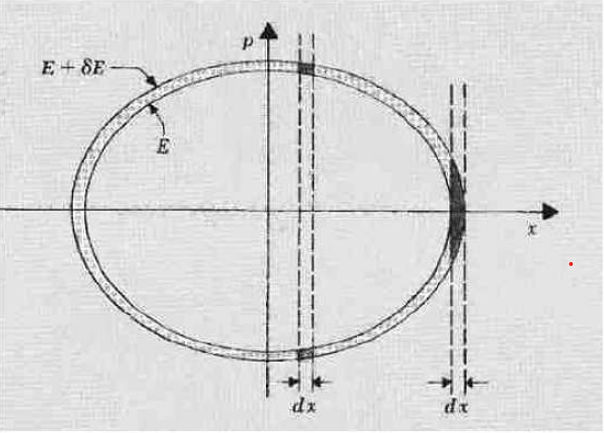
\includegraphics[width=10cm]{pic/2bab2.png}
                \caption{Deskripsi ruang fase partikel pada energi $E$ dan $E+\delta E$}
            \end{figure}
        \end{enumerate}
        \item Pandang persamaan berikut :
        \begin{equation*}
            A\,dx=B\,dy\equiv\dbar F
        \end{equation*}
        dengan $A$ dan $B$ masing-masing fungsi $X$ dan $y$
        \begin{enumerate}[(a)]
            \item Jika $\,\dbar F$ adalah diferensial eksak sehingga $F=F(x,y)$. Tunjukkan bahwa $A$ dan $B$ mengikuti 
            \begin{equation*}
                \dfrac{\partial A}{\partial y}=\dfrac{\partial B}{\partial x}
            \end{equation*}
            \item Jika $\dbar F$ adalah diferensial eksak, tunjukkan bahwa integral $\int \,\dbar F$ pada lintasan tertutup pada bidang $xy$ adalah nol.
        \end{enumerate}
    \end{enumerate}
\textbf{Tugas 3 (Bab 3)}
\begin{enumerate}
    \item Sebuah kotak dipisahkan menjadi dua bagian dengan rasio 3:1. Kotak besar mengandung 1000
    molekul gas Ne dan kotak kecil mengandung 100 molekul gas He. Sebuah lubang kecil
    dibuat antara kotak besar dan kecil dan sistem dalam kesetimbangan.
    \begin{enumerate}[(a)]
        \item Tentukan jumlah rata-rata molekul untuk setiap kotak
        \item Tentukan probabilitas dari 1000 molekul Ne dan 100 molekul Ne.
    \end{enumerate}
    \item Pandang ada sejumlah $N$ partikel dengan interaksi antar partikel diabaikan. Masing-masing partikel memiliki spin $\dfrac{1}{2}$ dan momen magnet $\mu$ dan medan magnet $H$
    \begin{enumerate}[(a)]
        \item Tentukan hubungan antara temperatur absolut $T$ dan energi total sistem $E$ menggunakan bentuk ekspresi $\beta\equiv\dfrac{\partial\ln\Omega}{\partial E}$
        \item Jika momen magnetik total adalah $M$ berkaitan dengan energi $E$. Tentukan parameter $M$ sebagai fungsi medan magnet $H$ dan temperatur $T$.
    \end{enumerate}
    \item Suatu sistem $A$ melakukan kontak termal dengan sebuah reservoir $A'$ pada temperatur $T'$. Kemudian sistem $A$ menyerap panas sejumlah $Q$ selama proses tersebut. Tunjukkan bahwa entropi $\Delta S$ pada sistem $A$ adalah $\Delta S\ge \dfrac{Q}{T'}$.
\end{enumerate}
\textbf{Tugas 4 (Bab 6)}
\begin{enumerate}
    \item Sebuah osilator harmonik 1 dimensi memiliki tingkat energi $E_n=(n+\dfrac{1}{2})\hbar\omega$ dengan $n$ adalah bilangan kuantum $(n=0, 1, 2,\dots)$ dan $\omega$ merupakan frekuesi angular. Jika osilator harmonik melakukan kontak termal dengan sebuah reservoir temperatur cukup rendah $T$ sehingga $\dfrac{kT}{\hbar\omega}\ll1$.
    \begin{enumerate}[(a)]
        \item Tentukan perbandingan probabilitas osilator harmonik pada tingkat pertama dengan tingkat dasar.
        \item Tentukan energi rata-rata dari osilator harmonik sebagai fungsi temperatur $T$ pada kondisi energi pertama dan dasar.
    \end{enumerate}
    \item Sebuah mineral minyak diletakkan pada medan magnet $H$. Setiap proton dari material memiliki spin $\dfrac{1}{2}$ dan momen magnet $\mu$. Energi proton memiliki dua keadaan yaitu $\epsilon=\mp\mu H$ dari orientasi spin. Sebuah gelombang radio diaplikasikan pada interval energi tersebut, jika frekuensi $\nu$ memenuhi kondisi Bohr $h\nu =2\nu H$. Daya yang diserap dari medan radiasi sebanding dengan perbedaan jumlah inti dari dua tingkat energi. Jika diasumsikan proton dari mineral minyak dalam keadaan kesetimbangan termal pada temperatur $T$ atau memenuhi kondisi $\nu H\ll kT$. Tentukan daya penyerapan mineral sebagai fungsi temperatur $T$.
    \item Pandang gas ideal dengan temperatur absolut $T$ didalam medan gravitasi yang uniform yang dijelaskan dengan percepatan $g$. Dengan menuliskan syarat kondisi kesetimbangan hidrostatik sebagai titik gas yang terletak diantara ketinggian $z$ dan $z+\,dz$, turunkan persamaan untuk $n(z)$ dan jumlah molekul per cm$^3$ pada ketinggian $z$. 
\end{enumerate}
\textbf{Tugas 5 (Bab 7)}
\begin{enumerate}
    \item  Sebuah gas ideal monoatomik terdiri atas $N$ partikel, masing-masing partikel bermassa $m$
    berada dalam kesetimbangan pada temperatur $T$. Gas berada dalam sebuah kotak dengan
    sisi-sisinya berukuran $L$ yang memiliki sisi bawah dan atas sejajar dengan permukaan bumi
    sehingga efek medan gravitasi $g$ pada partikel perlu diperhatikan
    \begin{enumerate}[(a)]
        \item Tentukan energi kinetik rata-rata partikel
        \item Tentukan energi potensial rata-rata partikel
    \end{enumerate}
    \item Sebuah wadah bersifat isolasi termal terdiri atas 2 bagian, masing-masing dipisahkan oleh sebuah bahan insulator. Kedua ruang berisi gas ideal memiliki kapasitas panas tetap $c_v$. Salah satu ruang memiliki jumlah $v_i$ mol dan temperatur $T_1$ dan tekanan $\bar{p}_1$ dan yang lain $v_2$ mol dan tempertaur $T_2$ dan tekanan $\bar{p}_2$. Kemudian pembatas antara 2 ruangan dihilangkan dan gas mencapai kesetimbangan
    \begin{enumerate}[(a)]
        \item Tentukan tekanan akhir
        \item Tentukan perubahan entropi $\Delta S$ jika tipe gas berbeda
    \end{enumerate} 
    \item Pandang ada sejumlah $N$ partikel dengan interaksi antar partikel diabaikan. Masing-masing
    partikel memiliki spin $\dfrac{1}{2}$ dan momen magnet $mu$ dalam medan magnet $H$. Dengan menuliskan kesetimbangan hidrostatis untuk gas yang terletak antara ketinggian $z$ dan $z+dz$, turunkan persamaan untuk $n(z)$ dan jumlah molekul per $cm^3$ pada ketinggian $z$
\end{enumerate}
    \title{\centering\Large{{\textbf{Jawaban}}}}\\\\
\textbf{Tugas 1}
\begin{enumerate}
    \item 
    \begin{enumerate}[(a)]
        \item 
        Probabilitas langkah $n_1$ ke kanan dan $n_2=N-n_1$ kekiri:
        \begin{equation*}
            W(n_1)=\dfrac{N!}{n_1!(N-n_1)!}p^{n_1}q^{N-n1}
        \end{equation*}
        Sehingga didapatkan persamaan binomial
        \begin{equation*}
            \sum_{n_1=0}^N W(n_1)=(p+q)^N =1
        \end{equation*}
        Untuk setiap fungsi $f(n_1)$ didapatkan
        \begin{equation*}
            \begin{split}
                \overline{f(n_1)}&=\dfrac{\sum_{n_1=0}^N W(n_1)f(n_1)}{\sum_{n_1=0}^N W(n_1)}\\
                &=\sum_{n_1=0}^N f(n_1)W(n_1)
            \end{split}
        \end{equation*}
        Dengan perpindahan rata-rata dari $m$:
        \begin{equation*}
            \begin{split}
                \overline{m}&=\overline{n_1-n_2}\\
                &=\sum_{n_1=0}^N (n_1-n_2)W(n_1)\\
                &=\sum_{n_1=0}^N\left(p\dfrac{\partial}{\partial p} -q \dfrac{\partial}{\partial q}\right)W(n_1)\\
                &=\left(p\dfrac{\partial}{\partial p} -q \dfrac{\partial}{\partial q}\right)\sum_{n_1=0}^N W(n_1)\\
                &=\left(p\dfrac{\partial}{\partial p} -q \dfrac{\partial}{\partial q}\right)(p+q)^N
            \end{split}
        \end{equation*}
        Dengan nilai $p=q=\dfrac{1}{2}$
        \begin{equation*}
            \begin{split}
                \overline{m}&=pN(p+q)^{N-1}-qN(p+q)^{N-1}\\
                &=N(p+q)^{N-1}(p-q)\\
                &=0
            \end{split}
        \end{equation*}
        Untuk mencari nilai rata-rata $m^2$ yang memiliki kemiripan dengan nilai $m$:
        \begin{equation*}
            \begin{split}
                \overline{m^2}&=\overline{(n_1-n_2)^2}\\
                &=\sum_{n_1=0}^N (n_1-n_2)^2 W(n_1)\\
                &=\sum_{n_1=0}^N \left(p\dfrac{\partial}{\partial p}-q \dfrac{\partial}{\partial q}\right)^2 W(n_1)\\
                &=\left(p\dfrac{\partial}{\partial p}-q \dfrac{\partial}{\partial q}\right)^2 \sum_{n_1=0}^N W(n_1)\\
                &=\left(p\dfrac{\partial}{\partial p} -q \dfrac{\partial}{\partial q}\right)(N(p+q)^{N-2}(p-q))
            \end{split}
        \end{equation*}
        Dengan nilai $p=q=\dfrac{1}{2}$
        \begin{equation*}
            \begin{split}
                \overline{m^2}&=pN(p+q)^{N-1}+pN(N-1)(p+q)^{N-2}(p-q)\\
                &\;\;\;\;-qN(N-1)(p+1)^{N-2}(p-q)+qN(p+q)^{N-1}\\
                &=N(p+q)^N+N(N-1)(p+q)^{N-2}(p-q)^2\\
                &=N\sum_{n_1=0}^N W(N_1)+N(N-1)(p+q)^{N-2}(p-q)^2\\
                &=N 
            \end{split}
        \end{equation*}
        \item Hitung rata-rata $\overline{m^3}$ dan $\overline{m^4}$.
        Mencari nilai $\overline{m^3}$
        \begin{equation*}
            \begin{split}
                \overline{m^3}&=\overline{(n_1-n_2)^3}\\
                &=\sum_{n_1=0}^N(n_1-n_2)^3W(n_1)\\
                &=\sum_{n_1=0}^N\left(p\dfrac{\partial}{\partial p}-q\dfrac{\partial}{\partial q}\right)^3W(n_1)\\
                &=\left(p\dfrac{\partial}{\partial p}-q\dfrac{\partial}{\partial q}\right)\overline{m^2}\\
                &=\left(p\dfrac{\partial}{\partial p}-q\dfrac{\partial}{\partial q}\right)\sum W(n_1)+N(N-1)(p+q)^N-2(p-q)^2\\
                &=N^2(p+q)^{N-1}(p-q)+N(N-1)(N-2)(p+q)^{N-3}(p-q)^3\\
                &\;\;\;+2N(N-1)(p+q)^{N-1}(p-q)\\
                &=\left[N+2(N-1)\overline{m}\right]+N(N-1)(N-2)(p+q)^{N-3}(p-q)^3\\
                &=\left[3N-2\overline{m}\right]+N(N-1)(N-2)(p+q)^{N-3}(p-q)^3
            \end{split}
        \end{equation*}
        Kemudian dengan p=q=$\dfrac{1}{2}$ maka didapat,
        \begin{equation*}
            \overline{m^3}=0
        \end{equation*}
        Sehingga nilai $\overline{m^4}$ didapat dengan:
        \begin{equation*}
            \begin{split}
                \overline{m^4}&=\sum_{n_1=0}^N (n_1-n_2)^4 W(n_1)\\
                &=\sum_{n_1=0}^N \left(p\dfrac{\partial}{\partial p}-q\dfrac{\partial}{\partial q}\right)^4 W(n_1)\\
                &=\left(p\dfrac{\partial}{\partial p}-q\dfrac{\partial}{\partial q}\right)\overline{m^3}\\
                &=\left(p\dfrac{\partial}{\partial p}-q\dfrac{\partial}{\partial q}\right)\left[3N-2\right]\overline{m}+N(N-1)(N-2)(p+q)^{N-3}(p-q)^3\\
                &=(3N-2)\overline{m^2}+3N(N-1)(N-2)(p+q)^{N-2}(p-q)^2\\
                &\;\;\;+N(N-1)(N-2)(N-3)(p+q)^{N-4}(p-q)^4
            \end{split}
        \end{equation*}
        dengan 
            \begin{equation*}
                N(N-1)(p+q)^{N-2}(p-q)^2=\overline{m^2}-N\sum W(n_1)
            \end{equation*}
        maka,
        \begin{equation*}
            \overline{m^4}=(6N-8)\overline{m^2}-(3N-6)N\sum W(n_1)+N(N-1)(N-2)(N-3)(p+q)^{N-4}(p-q)^4
        \end{equation*}
        Dengan nilai $p=q=\dfrac{1}{2}$ maka,
        \begin{equation*}
            \overline{m^4}=(3N-2)N
        \end{equation*}
    \end{enumerate}
    \item Dengan
    \begin{equation*}
        W(n)=\dfrac{N!}{n!(N-n)!}p^n(1-p)^{N-n}
    \end{equation*}
    \begin{enumerate}[(a)]
        \item Jika $\ln(1-p)\approx-p$. Tunjukkan $(1-p)^{N-n}$\\
        \begin{itemize}
            \item Dengan $n\ll N$ sehingga $N-n\approx N$
            \begin{equation*}
                (1-p)^{N-n}=(1-p)^N
            \end{equation*}
            \item Kemudian meninjau ruas kanan
            \begin{equation*}
                e^{(-Np)}
            \end{equation*}
        \end{itemize}
        Sehingga didapat:
        \begin{equation*}
        	\begin{split}
            (1-p)^N &\approx e^{(-Np)}\\
            \ln(1-p)^N &\approx \ln e^{(-Np)}\\
            N\ln(1-p) &\approx-Np
        	\end{split}
        \end{equation*}
        Dan dengan $\ln(1-p)\approx -p$, maka
        \begin{equation*}
            -Np\approx-Np
        \end{equation*}
        \begin{center}
            Q.E.D.
        \end{center}
        \item Tunjukkan bahwa $\dfrac{N!}{(N-n)!}\approx N^n$
        \begin{equation*}
            \begin{split}
                \dfrac{N!}{(N-n)!}&=\dfrac{N\times\cdots\times 3\times 2\times 1}{(N-n)\times\cdots\times 3\times2 \times 1}\\
                &=(N-n+1)\times (N-n+2)\times\cdots\times N
            \end{split}
        \end{equation*}
        Dengan $n\ll N$, sehingga:
        \begin{equation*}
            \begin{split}
                \dfrac{N!}{(N-n)!}&=(N-n+1)\times (N-n+2)\times\cdots\times N\\
            &=N^n+n^n+\cdots+(1^n-1)\\
            &=N^n
            \end{split}
        \end{equation*}
        \item Tunjukkan bahwa $W(n)=\dfrac{\lambda^n}{(n!)e^{-\lambda}}$ dengan $\lambda=Np$ dikenal sebagai distribusi Poisson.\\\\
        Dengan definisi distribusi Binomial
        \begin{equation*}
            \begin{split}
                W(n)&=\dfrac{N!}{n!(N-n)!}p^n(1-p)^{N-n}\\
                &=\dfrac{N(N-1)\cdots(N-n+1)}{n!}p^n(1-p)^{N-n}\\
                &=\dfrac{N^n\left(1-\dfrac{1}{N}\right)\left(1-\dfrac{2}{N}\right)\cdots\left(1-\dfrac{n-1}{N}\right)}{n!(N-n)!}p^n(1-p)^{N-n}\\
                &=\dfrac{\left(1-\dfrac{1}{N}\right)\left(1-\dfrac{2}{N}\right)\cdots\left(1-\dfrac{n-1}{N}\right)}{n!(N-n)!}(Np)^n\left(1-\dfrac{Np}{N}\right)
            \end{split}
        \end{equation*}
        Ketika nilai $p\gg$ dan $N\ll$, maka:
        \begin{equation*}
            W(n)=e^{-Np}\dfrac{(Np)^n}{n!}
        \end{equation*}
        Dengan $\lambda=Np$ yang merupakan definisi distribusi Poisson, maka:
        \begin{equation*}
            W(n)=e^{-\lambda}\dfrac{\lambda^n}{n!}
        \end{equation*}
    \end{enumerate}
    \item 
    \begin{enumerate}[(a)]
        \item Mengambil batas distribusi binomial
        \begin{equation*}
            \begin{split}
                \sum W_n&=\sum \dfrac{\lambda^ne^{-\lambda}}{n!}\\
                &=e^{-\lambda} \sum \dfrac{\lambda^n}{n!}\\
                &=e^{-\lambda}e^{\lambda}\\
                &=1\;\;\;\text{terbukti}
            \end{split}
        \end{equation*}
        \item Distribusi poisson berasal dari distribusi binomial
        \begin{equation*}
            \bar{n}=np
        \end{equation*}
        \item 
        \begin{equation*}
            \begin{split}
                \bar{\Delta n^2}&=\bar{n-\bar{n}}^2\\
                &=\bar{n-np}^2\\
                &=\bar{n^2(1-p)^2}\\
                &=\sum_{n=0^N} n^2(1-p)^2W(n)
            \end{split}
        \end{equation*}
    \end{enumerate}
\end{enumerate}
    \textbf{Tugas 2}
\begin{enumerate}
    \item Hamiltonian: $H(x,p)=\dfrac{p^2}{2m}+\dfrac{1}{2}kx^2=E$
    \begin{equation*}
        \begin{split}
            \rightarrow\;H(0,p)&=\dfrac{p^2}{2m}=E\\
            p&=\sqrt{2mE}\\
            H(L,p)&=\dfrac{p^2}{2m}+\dfrac{1}{2}kL^2=E\\
            p&=\sqrt{\dfrac{2mE}{p^2+mkL^2}}
        \end{split}
    \end{equation*}
    dengan 1 dimensi $\rightarrow$ 1N
    \begin{equation*}
        \begin{split}
            \Delta\omega&=\int_{E\ll H\ll E\delta E} dxdx=\int_{E\ll H\ll E\delta E} d\omega\\
            \omega&=\int_{E\ll H\ll E\delta E}L\,dp\\
            &=\int_{\sqrt{2mE}}^{\sqrt{\sfrac{2mE}{p^2+mkL^2}}}Ldp\\
            &=L\left(\sqrt{2mE}\right)\left(\dfrac{1-\sqrt{p^2+mkL^2}}{\sqrt{p^2+mkL^2}}\right)
        \end{split}
    \end{equation*}
    \item 
    \begin{enumerate}[(a)]
        \item dengan probabilitas ensembel
        \begin{equation*}
            P(x)dx=\sum\dfrac{W(\varphi) d\varphi}{\sfrac{dx}{d\varphi}}
        \end{equation*}
        dengan persamaan gemolmbang osilator harmonik
        \begin{equation*}
            \dfrac{dx}{d\varphi}=A\sin(\omega t+\varphi)
        \end{equation*}
        maka,
        \begin{equation*}
            \omega=(\varphi)d\varphi=\dfrac{d\varphi}{2\pi}
        \end{equation*}
        sehingga didapatkan,
        \begin{equation*}
            \begin{split}
                P(x)dx&=\sum\dfrac{W(\varphi) d\varphi}{\sfrac{dx}{d\varphi}}\\
                &=\dfrac{2dx}{2\pi A\sin(\omega t+\varphi)}\\
                &=\dfrac{1}{\pi\sqrt{A^2-x^2}}dx
            \end{split}
        \end{equation*}
        \item Dengan
        \begin{equation*}
            \begin{split}
                x&=A\cos(\omega t+\varphi)\\
                \dfrac{dx}{d\varphi}&=A\sin(\omega t+\varphi)
            \end{split}
        \end{equation*}
        dan dengan
        \begin{equation*}
            \omega(\varphi)\,d\varphi=(2\pi)^{-1}\,d\varphi
        \end{equation*}
        Sehingga didapatkan
        \begin{equation*}
            \begin{split}
                p(x)dx&=\dfrac{2\,dx}{2\pi A\sin(\omega t+\varphi)}\\
                &=\dfrac{1}{\pi\sqrt{A^2-x^2}}\,dx
            \end{split}
        \end{equation*}
        \item Energi sebagai fungsi dari amplitudo
        \begin{equation*}
            \begin{split}
                E&=\dfrac{p^2}{2m}+\dfrac{kx^2}{2}\\
                &=\dfrac{kA^2}{2}
            \end{split}
        \end{equation*}
        Dengan kontur energi pada fase ruang sebanding dengan elips.\\
        Dengan transformasi
        \begin{equation*}
            p\prime^2=\dfrac{p^2}{mk}
        \end{equation*}
        maka didapat lingkaran sebagai kontur energi, sehingga:
        \begin{equation*}
            \rightarrow A^2=x^2+p\prime^2 
        \end{equation*}
        dengan fase ruang volume berada diandata $E$ dan $E+\delta E$ yang direpresentasikan dengan luas $a$ diantara $A$ dan $A+\delta A$ dimana $\delta A$ merupakan fungsi
        \begin{equation*}
            \omega(A)\delta A=2\pi A\delta A
        \end{equation*}
        Untuk menemukan dimana bagian dari ruang fase diantara $x$ dan $dx$, gunakan koordinat polar
        \begin{equation*}
            \begin{split}
                \cos\theta&=\dfrac{x}{A}\\
                d\theta&=\dfrac{dx}{A\sin\theta}=\dfrac{dx}{\sqrt{A^2-x^2}}
            \end{split}
        \end{equation*}
        Sehingga area diantara dua bagian antara $x$ dan $dx$ adalah
        \begin{equation*}
            \begin{split}
                \omega(x,A)\,dx\delta A&=2A\,d\theta\delta A\\
                &=\dfrac{2A\,dx\delta A}{\sqrt{A^2-x^2}}
            \end{split}
        \end{equation*}
        dan probabilitasnya dalah
        \begin{equation*}
            \begin{split}
                P(x)dx&=\dfrac{\omega(x,A)dx\delta A}{\omega(A)\delta A}\\
                &=\dfrac{dx}{\pi\sqrt{A^2-x^2}}
            \end{split}
        \end{equation*}
    \end{enumerate}
    \item 
    \begin{enumerate}[(a)]
        \item 
        \begin{equation*}
            \begin{split}
                F&=F(x,y)\\
                dF&=\dfrac{\partial F}{\partial x}\,dy+\dfrac{\partial F}{\partial y}\,dy\\
                \leadsto&\,\,dF=A\,dx+B\,dy
            \end{split}
        \end{equation*}
        dengan
        \begin{equation*}
            A=\dfrac{\partial F}{\partial x}
        \end{equation*}
        maka, 
        \begin{equation*}
            \dfrac{\partial A}{\partial y}=\dfrac{\partial^2 F}{\partial x\partial y}
        \end{equation*}
        dan 
        \begin{equation*}
            B=\dfrac{\partial F}{\partial y}
        \end{equation*}
        maka,
        \begin{equation*}
            \dfrac{\partial B}{\partial x}=\dfrac{\partial^2 F}{\partial x\partial y}
        \end{equation*}
        sehingga 
        \begin{equation*}
            \dfrac{\partial A}{\partial y}=\dfrac{\partial B}{\partial x}
        \end{equation*}
        \item 
        \begin{equation*}
            \begin{split}
                \int_A^B \,dF&=F(B)-F(A)\\
                &=F(x_N,y_N)- F(x_0,y_0)
            \end{split}
        \end{equation*}
        Lintasan tertutup, maka $X_N\rightarrow X_0$ dan $y_N\rightarrow y_0$
        \begin{equation*}
            \begin{split}
                \oint\,df&=\int_A^B\,dF\\
                &=F(x_0,y_0)- F(x_0,y_0)\\
                &=0
            \end{split}
        \end{equation*}
    \end{enumerate}
\end{enumerate}
    \textbf{Tugas 3}
\begin{enumerate}
    \item  
    \begin{enumerate}[(a)]
        \item Jumlah rata-rata molekul untuk setiap kotak\\
        Pada kotak besar
        \begin{itemize}
            \item jumlah Ne $=1000\times\dfrac{3}{4}=750$ molekul
            \item jumlah He $=100\times\dfrac{3}{4}=75$ molekul
        \end{itemize}
        Pada kotak kecil
        \begin{itemize}
            \item jumlah Ne $=1000\times\dfrac{1}{4}=250$ molekul
            \item jumlah He $=100\times\dfrac{1}{4}=25$ molekul
        \end{itemize}
        \item Probabilitas dari 1000 molekul Ne dan 100 molekul N
        \begin{itemize}
            \item molekul Ne pada kotak besar:
            \begin{equation*}
                P_{Ne}=\left(\dfrac{3}{4}\right)^{1000}
            \end{equation*}
            \item molekul Ne pada kotak besar:
            \begin{equation*}
                P_{Ne}=\left(\dfrac{1}{4}\right)^{100}
            \end{equation*}
        \end{itemize}
    \end{enumerate}
    \item 
    \begin{enumerate}[(a)]
        \item Nilai mikrostate
        \begin{equation*}
            \Omega(N,n_{\uparrow})=\dfrac{N!}{n_{\uparrow}!(N-n_{\uparrow})}
        \end{equation*}
        dengan energi medan magnet
        \begin{equation*}
            \begin{split}
                E&=(N-2n_{\uparrow})\mu B\;\;\;\leadsto H=\dfrac{B}{\mu}\\
                &=(N-2n_{\uparrow})\mu^2 B
            \end{split}
        \end{equation*}
        dengan entropi
        \begin{equation*}
            S=k_B\ln\Omega=k_B\ln\left[\dfrac{N!}{n_{\uparrow}!(N-n_{\uparrow})}\right]\leadsto n_{\uparrow}=\dfrac{1}{2}\left(N-\dfrac{E}{\mu^2 H}\right)
        \end{equation*}
        dari formula stirling
        \begin{equation*}
            S=k_B\left[N\ln N-n_{\uparrow}\ln n_{\uparrow}-(N-n_{\uparrow})\ln(N-n_{\uparrow})\right]
        \end{equation*}
        dan dari relasi termodinamik
         \begin{equation*}
             \begin{split}
                 dE&=TdS-mdB\\
                 dS&=\dfrac{1}{T}dE+\dfrac{m}{T}dB
             \end{split}
         \end{equation*}
         Sehingga didapatkan:
         \begin{equation*}
            \begin{split}
                \left(\dfrac{\partial S}{\partial E}\right)&=\dfrac{1}{T}\\
                k_B\dfrac{\partial \ln\Omega}{\partial E}&=\dfrac{1}{T}\;\;\;\leadsto\beta=\dfrac{\partial \ln\Omega}{\partial E}\\
                k_B\beta&=\dfrac{1}{T}
            \end{split}
         \end{equation*}
         maka,
         \begin{equation*}
             \begin{split}
                \dfrac{1}{T}&=k_B\left[-\ln n_{\uparrow}-1+\ln(N-n_{\uparrow}+1)\right]\left(-\dfrac{1}{2\mu^2H}\right)\\
                &=k_B\left[-\ln \left(\dfrac{1}{2}\left(N-
                \dfrac{E}{\mu^2H}\right)\right)+\ln\left(N-\dfrac{1}{2}\left(N-
                \dfrac{E}{\mu^2H}\right)\right)\right]\left(-\dfrac{1}{2\mu^2H}\right)
             \end{split}
         \end{equation*}
         \item 
         \begin{equation*}
            dS=\dfrac{1}{T}dE+\dfrac{M}{T} 
         \end{equation*}
         kemudian didapatkan
        \begin{equation*}
            \left(\dfrac{\partial S}{\partial B}\right)=\dfrac{M}{T}
        \end{equation*}
        maka,
        \begin{equation*}
            \begin{split}
                \dfrac{M}{T}&=k_B\left[-\ln \left(\dfrac{1}{2}\left(N-
                \dfrac{E}{\mu^2H}\right)\right)+\ln\left(N-\dfrac{1}{2}\left(N-
                \dfrac{E}{\mu^2H}\right)\right)\right]\left(\dfrac{E}{2\mu^3H^2}\right)\\
                M(H,T)&=k_BT\left[-\ln \left(\dfrac{1}{2}\left(N-
                \dfrac{E}{\mu^2H}\right)\right)+\ln\left(N-\dfrac{1}{2}\left(N-
                \dfrac{E}{\mu^2H}\right)\right)\right]\left(\dfrac{E}{2\mu^3H^2}\right)
            \end{split}
        \end{equation*}
    \end{enumerate}
    \item Perubahan entropi diberikan oleh:
    \begin{equation*}
        \Delta S=\int dS=\int \dfrac{dQ}{T}
    \end{equation*}
    Dengan sistem $A$ berada pada temperatur lebih rendah dari sistem $A\prime$, sehingga 
    \begin{equation*}
        Q>0\;\;\;\text{dan}\;\;\;T\leq T\prime
    \end{equation*}
    maka didapat:
    \begin{equation*}
        \begin{split}
            \Delta S&=\int \dfrac{dQ}{T}>\int\dfrac{dQ}{T\prime}\\
            &=\dfrac{Q}{T\prime}
        \end{split}
    \end{equation*}
    karena $T\prime$ konstan untuk reservoir panas, maka didapat:
    \begin{equation*}
        \Delta S\geq \dfrac{Q}{T\prime}
    \end{equation*}
\end{enumerate}
    \textbf{Tugas 4}
\begin{enumerate}
    \item \begin{enumerate}[(a)]
        \item 
        \begin{equation*}
            \dfrac{P_1}{P_2}=\dfrac{e^{-\beta E_1}}{e^{-\beta E_0}}=\dfrac{e^{-\beta(1+\sfrac{1}{2})\hbar\omega}}{e^-\beta(0+\sfrac{1}{2})\hbar\omega}
        \end{equation*}
        \item 
        \begin{equation*}
            \begin{split}
                \bar{E}&=\dfrac{\sum_re^{-\beta E_r}E_r}{\sum_r e^{-\beta E_r}}=\dfrac{E_oe^{-\beta E_o}+E_1e^{-\beta E_1}}{e^{-\beta E_o}+e^{-\beta E_1}}\\
                &=\hbar\omega\dfrac{\dfrac{1}{2}+\dfrac{3}{2}\dfrac{P_1}{P_0}}{1+\dfrac{P_1}{P_0}}=\dfrac{\hbar\omega}{2}\dfrac{1+3e^{-\beta\hbar\omega}}{1+e^{-\beta\hbar\omega}}
            \end{split}
        \end{equation*}
    \end{enumerate}
    \item Melabeli proton dengan indeks $i$, dengan $i$ berjalan dari 1 ke $N$, dan spin proton bernilai $s_i\mu$. Dengan energi state $\sum_i(-s_i\mu H)$, maka fungsi partisinya adalah
    \begin{equation*}
        Z(T)=\sum_{s_1,\cdots,s_N} e^{\sfrac{1}{kT}\sum_i s_i\mu H}
    \end{equation*}
    dimana
    \begin{equation*}
        \begin{split}
            Z(T)&=(Z_1(T))^N\\
            Z_1(T)&=e^{-\sfrac{\mu H}{kT}}+e^{\sfrac{\mu H}{kT}}
        \end{split}
    \end{equation*}
    Energi internal dari sampel $U=-\sum_i s_i\mu H$ sebanding dengan perbedaan populasi. Sehingga didapat:
    \begin{equation*}
        U=kT^2 \dfrac{\partial}{\partial T} \log(Z(T))
    \end{equation*}
    sehingga didapat
    \begin{equation*}
    	U=kT^2N\dfrac{e^{+\sfrac{\mu H}{kT}}-e^{-\sfrac{\mu H}{kT}}}{e^{+\sfrac{\mu H}{kT}}+e^{-\sfrac{\mu H}{kT}}}\left(\dfrac{-\mu H}{kT^2}\right)
    \end{equation*}
    Dimana ketika $\mu H\ll kT$ mengganti eksponen dengan $e^x=1+x$ sehingga didapatkan
    \begin{equation*}
        \begin{split}
            U&\approx-N\mu H\dfrac{+\sfrac{\mu H}{kT}-\left(\sfrac{\mu H}{kT}\right)}{2}\\
            &=-N\dfrac{\mu^2H^2}{kT}
        \end{split}
    \end{equation*}
    dan daya berbanding terbalik dengan $T$
    \item $PV=nRT$ dapat ditulis $P=\dfrac{\rho}{\mu}RT$ dengan $\mu$ adalah berat molekul\\
    Dengan kesetimbangan hidrostatis: $\dfrac{dP}{dt}=-q\rho$, sehingga
    \begin{equation*}
        \begin{split}
            \dfrac{dP}{dz}=-\dfrac{q\mu}{RT}P\\
            \rightarrow \dfrac{dP}{P}=-\dfrac{g\mu}{RT}dz
        \end{split}
    \end{equation*}
    sehingga:
    \begin{equation*}
        \begin{split}
            \ln P&=-\dfrac{\mu g}{RT}z\\
            \rightarrow \ln P&=P_0 e^{-\dfrac{g\mu}{RT}z}\\
            \ln P+z\dfrac{g\mu}{RT}&=0\rightarrow \dfrac{dN(z)}{dz}=\dfrac{\mu g}{RT}\\
            \ln P+z\dfrac{g\mu}{RT}&=N(z)+z\dfrac{dN(z)}{dz}
        \end{split}
    \end{equation*}
\end{enumerate}
    \textbf{Tugas 5}
\begin{enumerate}
    \item 
    \begin{enumerate}[(a)]
        \item Dari teorema equipartisi didapatkan
        \begin{equation*}
            \begin{split}
                \langle EK \rangle&=\dfrac{1}{2}mv_x ^2+\dfrac{1}{2}mv_y ^2+\dfrac{1}{2}mv_z ^2\\
                &=\dfrac{3}{2}k_BT
            \end{split}
        \end{equation*}
        \item Energi potensial rata-rata partikel
        \begin{equation*}
            \langle EP \rangle =\int_0^L\dfrac{mgze^{-\sfrac{mgz}{k_BT}}dz}{e^{-\sfrac{mgz}{k_BT}}dz}=\dfrac{I_N}{I_D}
        \end{equation*}
        dengan
        \begin{equation*}
            \begin{split}
                \rightarrow I_D&=\int_0^L e^{-\dfrac{mgz}{k_BT}}dz=\int_0^L e^{-\alpha z}dz=\left(\dfrac{1-e^{-\alpha z}}{\alpha}\right)\\
                \rightarrow I_N&=\int_0^L (mgz)e^{-\sfrac{mgz}{k_BT}}dz=mg\int_0^L ze^{-\sfrac{mgz}{k_BT}}dz\\
                &=-mh\dfrac{\partial I_D}{\partial \alpha}=\dfrac{mg}{\alpha}\left[\dfrac{1-e^{-\alpha L}}{\alpha}-Le^{-\alpha L}\right]
            \end{split}
        \end{equation*}
        Sehingga didapatkan:
        \begin{equation*}
            \begin{split}
                \langle EK \rangle&=\dfrac{I_N}{I_D}=mg\left[\dfrac{1}{\alpha}-Le^{-\alpha L}\right]\\
                &=mg\left[\dfrac{k_BT}{mg}-
                \dfrac{L}{e^{\sfrac{mgL}{k_BT}}-1}\right]
            \end{split}
        \end{equation*}
    \end{enumerate}
    \item 
    \begin{enumerate}[(a)]
        \item 
            \begin{equation*}
            \bar{p_f}=\bar{p_1}+\bar{p_2}
            \end{equation*}
    \item Volume fasa ruang
    \begin{equation*}
        \Omega(E)=\dfrac{1}{N_1!N_2!}\dfrac{1}{h^{3N}}\int dq\int\prod_{i=1}^{3N_1}dp_i\int\prod_{j=1}^{3N_2}dp_j \theta(E-H(p_i,q_j))
    \end{equation*}
    Transformasi momentum
    \begin{equation*}
        \begin{split}
            P_1&\rightarrow P_i=\dfrac{P_i}{\sqrt{2m_1}}\leadsto dp_i=\sqrt{2m_1}\,dp_i\\
            P_2&\rightarrow P_j=\dfrac{P_j}{\sqrt{2m_2}}\leadsto dp_j=\sqrt{2m_2}\,dp_j
        \end{split}
    \end{equation*}
    maka,
    \begin{equation*}
        \begin{split}
            \Omega&=\dfrac{V^N(2m_1)^{\sfrac{3N_1}{2}}(2m_2)^{\sfrac{3N_2}{2}}}{h^{3N}N_1!N_2!}\int\prod_{i=1}^{3N}\,dp_i\theta\left(E-\sum_{i=1}^{3N}p_i ^2\right)\\
            &=\dfrac{V^N(2m_1)^{\sfrac{3N_1}{2}}(2m_2)^{\sfrac{3N_2}{2}}}{h^{3N}N_1!N_2!}\dfrac{\pi^{\sfrac{3N_1}{2}}E^{\sfrac{3N_1}{2}}}{\left(\dfrac{3N}{2}\right)!}
        \end{split}
    \end{equation*}
    dengan faktor massa reduksi $\mu=\dfrac{m_1m_2}{m_1+m_2}$
    \begin{equation*}
        \Omega=\dfrac{V^N\pi^{\sfrac{3N_1}{2}}(2\mu E)^{\sfrac{3N_2}{2}}}{h^{3N}N_1!\left(\dfrac{3N}{2}\right)!}\dfrac{N!}{N_1!N_2!}\left(\dfrac{m_1}{\mu}\right)^{\sfrac{3N_1}{2}}\left(\dfrac{m_2}{\mu}\right)^{\sfrac{3N_1}{2}}
    \end{equation*}
    Entropinya:
    \begin{equation*}
        \begin{split}
            S&=k_B\ln\Omega\\
            &=k_B\left[\ln\Omega_{\text{individu}}+\ln\Omega_{\text{campuran}}\right]\\
            &=S_{\text{individu}}+S_{\text{campuran}}
        \end{split}
    \end{equation*}
    maka:
    \begin{equation*}
        \dfrac{S_{\text{individu}}}{Nk_B}=\ln\left[\dfrac{V}{N}\left(\dfrac{4\pi\mu E}{3h^2N}\right)^{\sfrac{3}{2}}\right]+\dfrac{5}{2}
    \end{equation*}
    Untuk gas 1 dengan massa tereduksi
    \begin{equation*}
        \dfrac{S_{N_1}}{N_1k_B}=\ln\left[\dfrac{V}{N}\left(\dfrac{4\pi m_1 E}{3h^2N}\right)^{\sfrac{3}{2}}\right]+\dfrac{5}{2}+\ln\left(\dfrac{m_1}{\mu}^{\sfrac{3}{2}}\right)
    \end{equation*}
    Untuk gas 2
    \begin{equation*}
        \dfrac{S_{N_1}}{N_1k_B}=\ln\left[\dfrac{V}{N}\left(\dfrac{4\pi m_2 E}{3h^2N}\right)^{\sfrac{3}{2}}\right]+\dfrac{5}{2}+\ln\left(\dfrac{m_2}{\mu}^{\sfrac{3}{2}}\right)
    \end{equation*}
    Dan $\Delta S$ Entropinya
    \begin{equation*}
        \begin{split}
            \Delta S&=S_{\text{individu}}+S_{\text{campuran}}-S_{N_1}-S_{N_2}\\
            \dfrac{\Delta S}{k_B}&=-N_1\ln\dfrac{N_1}{N}-N_2\ln\dfrac{N_2}{N}
        \end{split}
    \end{equation*}
    \end{enumerate}
    \item $PV=nRT$ dapat ditulis $P=\dfrac{\rho}{\mu}RT$ dengan $\mu$ adalah berat molekul\\
    Dengan kesetimbangan hidrostatis: $\dfrac{dP}{dt}=-q\rho$, sehingga
    \begin{equation*}
        \begin{split}
            \dfrac{dP}{dz}=-\dfrac{q\mu}{RT}P\\
            \rightarrow \dfrac{dP}{P}=-\dfrac{g\mu}{RT}dz
        \end{split}
    \end{equation*}
    sehingga:
    \begin{equation*}
        \begin{split}
            \ln P&=-\dfrac{\mu g}{RT}z\\
            \rightarrow \ln P&=P_0 e^{-\dfrac{g\mu}{RT}z}\\
            \ln P+z\dfrac{g\mu}{RT}&=0\rightarrow \dfrac{dN(z)}{dz}=\dfrac{\mu g}{RT}\\
            \ln P+z\dfrac{g\mu}{RT}&=N(z)+z\dfrac{dN(z)}{dz}
        \end{split}
    \end{equation*}
\end{enumerate}
    
\end{document}
